\documentclass{article}
\usepackage{siunitx}
\usepackage{setspace}
\usepackage{gensymb}          
\usepackage{xcolor}
\usepackage{caption}
%\usepackage{subcaption}
%\doublespacing               
\singlespacing   
\usepackage[none]{hyphenat}   
\usepackage{amssymb} 
%\usepackage{relsize} 
\usepackage[cmex10]{amsmath}  
\usepackage{mathtools}      
\usepackage{amsmath}   
\usepackage{commath}  
%\usepackage{amsthm}    
%\interdisplaylinepenalty=2500 
%\savesymbol{iint}   
%\usepackage{txfonts}
%\restoresymbol{TXF}{iint}  
%\usepackage{wasysym}    
\usepackage{amsthm}   
\usepackage{mathrsfs}
\usepackage{txfonts}
\let\vec\mathbf{}
%\usepackage{stfloats}
\usepackage{float}
\usepackage{cite}
\usepackage{cases}
\usepackage{subfig}
%\usepackage{xtab}
\usepackage{longtable}
\usepackage{multirow}
%\usepackage{algorithm}
\usepackage{amssymb}
%\usepackage{algpseudocode}
\usepackage{enumitem}
\usepackage{mathtools}
%\usepackage{eenrc}
%\usepackage[framemethod=tikz]{mdframed}
\usepackage{listings}
\usepackage{listings}         
\usepackage[latin1]{inputenc}   
%% \usepackage{color}        
%% \usepackage{lscape}       
\usepackage{titling}                 
%\usepackage{fulbigskip}   
\usepackage{tikz}      
\usepackage{graphicx}
\graphicspath{{/Internal storage/Download/FWC
}}
\usepackage{atbegshi}
%http://ctan.org/pkg/atbegshi
\AtBeginDocument{\AtBeginShipoutNext{\AtBeginShipoutDiscard}}
%
\begin{document}
\begin{center}
\title{CHAPTER 9\\Areas of Parallelogram and Triangles}
\date{}
\maketitle
\section{EXERCISE 9.9.3}     
\end{center}
\begin{enumerate}
\item In fig.\ref{Fig.9.11}, $PSDA$ is a Parallelogram. Points $\vec{Q}$ and $\vec{R}$ are taken on $PS$ such that $PQ = QR = RS$ and $PA \parallel QB \parallel RC$. Prove that $ar (PQE) = ar (CFD)$.
\begin{figure}[h]
	\centering
	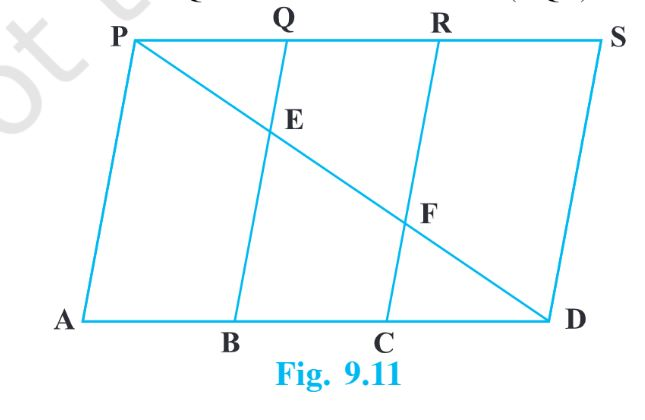
\includegraphics[width=\columnwidth]{Figures/Fig. 9.11.jpg}
	\caption{}
	\label{Fig.9.11}
\end{figure}
\item $\vec{X}$ and $\vec{Y}$ are on the side $LN$ of the triangle $LMN$ such that $LX = XY = YN$. Through $\vec{X}$, a line is drawn parallel to $LM$ to meet $MN$ at $\vec{Z}$ (See fig.\ref{Fig.9.12}). Prove that $ar (LYZ) = ar (MZYX)$
\begin{figure}[h]
	\centering
	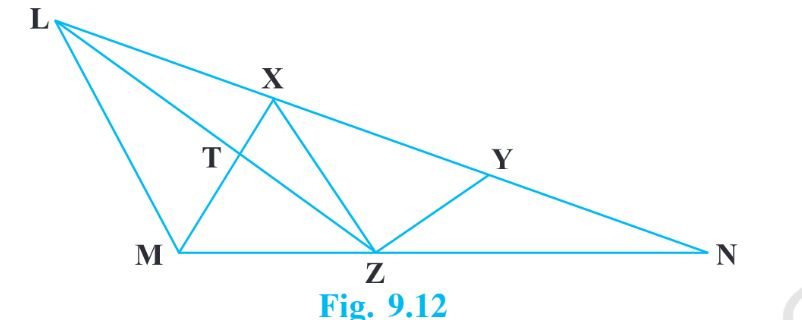
\includegraphics[width=\columnwidth]{Figures/Fig. 9.12.jpg}
	\caption{}
	\label{Fig.9.12}
\end{figure}
\item The area of the parallelogram $ABCD$ is $90cm^2$ (See fig.\ref{Fig.9.13}). Find
\begin{enumerate}
\item $ar (ABEF)$
\item $ar (ABD)$
\item $ar (BEF)$
\end{enumerate}
\begin{figure}[h]
          \centering{}
	  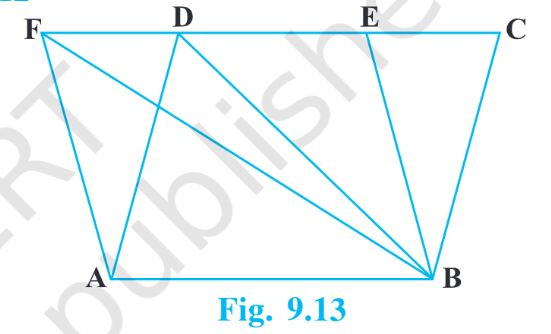
\includegraphics[width=\columnwidth]{Figures/Fig. 9.13.jpg}
	  \caption{}
	  \label{Fig.9.13}
\end{figure}
\item In $ \triangle ABC $, $\vec{D}$ is the mid-point of $AB$ and $\vec{P}$ is any point on $BC$. If $CQ \parallel PD$ meets $AB$ in $\vec{Q}$ (fig.\ref{Fig.9.14}), then prove that $ar (BPQ) = \frac{1}{2} ar(ABC).$
\begin{figure}[h]
	 \centering
	 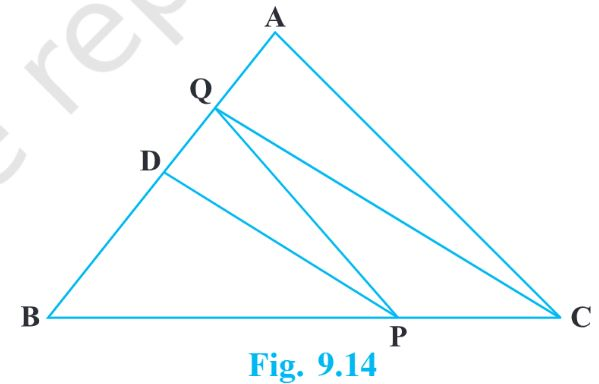
\includegraphics[width=\columnwidth]{Figures/Fig 9.14.jpg}
	 \caption{}
	 \label{Fig.9.14}
\end{figure}
\item $ABCD$ is a square. $\vec{E}$ and $\vec{F}$ are respectively the mid-points of $BC$ and $CD$. If $\vec{R}$ is the mid-point of $EF$ (fig.\ref{Fig.9.15}), Prove that $ar (AER) = ar(AFR)$
\begin{figure}[h]	
	\centering
	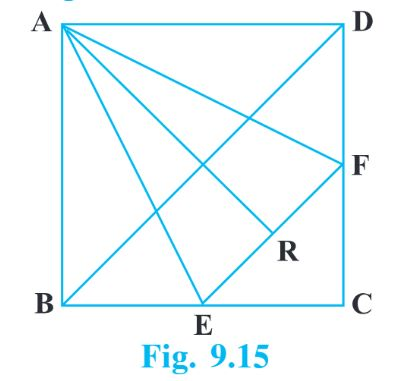
\includegraphics[width=\columnwidth]{Figures/Fig. 9.15.jpg}
	\caption{}
	\label{Fig.9.15}
\end{figure}
\end{enumerate}
\end{document}
